\hypertarget{fixed-wheel}{%
\section{Fixed Wheel}\label{fixed-wheel}}

We begin with the axle and wheel. Let P be the chassis center, L is the
distance from P to the wheel contact point. Define \(\alpha\) as the
angle between the wheel axle and \(X_R\) and \(\beta\) as the angle
between the wheel axis \(A\) and the axle. We also define \(A\) as the
vector in the wheel axle direction and \(v\) as the orthogonal vector
(the vector in the travel direction of the wheel). See
\texttt{wheelconfig}.

\begin{quote}
Basic wheel and axle configuration.
\end{quote}

\[A = \left\langle \cos(\alpha+\beta) , \sin(\alpha+\beta) \right\rangle\]

\[v = \left\langle \sin(\alpha+\beta) , -\cos(\alpha+\beta) \right\rangle\]

We will examine the linear and rotational aspects of motion separately.
They can be combined in the following manner:

\[\left\langle \dot{x}_I , \dot{y}_I , 0 \right\rangle + \left\langle 0 , 0 , \dot{\theta} \right\rangle =
\left\langle \dot{x}_I , \dot{y}_I , \dot{\theta} \right\rangle = \dot{\xi}_I\]

These equations are in the inertial or global coordinate system. Our
derivations will start in the robot or local coordinate system and so
the velocity vectors will need to be rotated into the robot coordinates:
\(\dot{\xi}_R = R(\theta)^{-1}\dot{\xi}_I\).

Recall earlier we introduced the \emph{no slip} and \emph{no slide}
constraints. Here we will apply the two constraints to derive the
fundamental kinematic equations for each wheel. Those equations will be
combined to build the equations of motion for the particular drive
system and hence the vehicle.

We begin with the no slip constraint. All of the motion of the vehicle
must be accounted for by wheel motion. This means that the total motion
of the craft must be equal to the wheel travel and in the wheel
direction. This seems obvious and can be translated into a mathematical
constraint using the no slip condition. First, we resolve the linear
motion of the craft and then address the rotational aspect. Recall that
magnitude of the linear motion from the wheel ( in the direction of the
wheel) is \(r\dot{\phi}\). The direction of motion is given by \(v\).
Since we have both linear and rotational motion built into
\(\dot{\xi}\), and to keep the dimensions matching up, the vector \(v\)
is extended to \(\langle v_1, v_2, 0 \rangle\). If \(v\) is a unit
vector, \(\| v \| = 1\), then the projection onto \(v\) is

\[P^1_v (u) = \frac{v\cdot u}{\| v\|^2} = v \cdot u = \left\langle \sin(\alpha+\beta) , -\cos(\alpha+\beta) , 0 \right\rangle \cdot u.\]\[Motion in the angular direction is shown by the vector :math:`w`.\]

For angular motion, we can break the motion of the wheel vector (\(v\))
into radial and angular components, \texttt{fig:angularradialmotion}.
The radial component is in the direction of the \(L\) vector. The
angular component is \(w\). It is the angular and not the radial
component which will contribute to \(\dot{\theta}\). The angular
component must have \(-L \dot{\theta}\) for the angular speed in the
\(w\) direction. {[}The negative comes from the direction of \(w\).{]}
Projecting that speed onto \(v\) gives \(-L\cos(\beta) \dot{\theta}\)
which means our projection component is
\(P^2_v = \left\langle 0 , 0 ,  -L\cos(\beta) \right\rangle\). Combining
the projections \(P_v = P^1_v + P^2_v\):

\[P_v =  \left\langle \sin(\alpha+\beta) , -\cos(\alpha+\beta), -L\cos(\beta) \right\rangle\]

and recall

\[P_v [\dot{\xi}_R]  = P_v [R(\theta)^{-1}\dot{\xi}_I] .\]

So we obtain:\\
\(P_v [R(\theta)^{-1}\dot{\xi}_I]\)

\[= \left\langle \sin(\alpha+\beta) , -\cos(\alpha+\beta), -L\cos(\beta) \right\rangle
\cdot R(\theta)^{-1}\left\langle \dot{x}_I , \dot{y}_I , \dot{\theta} \right\rangle .\]

For \emph{No Slip} we have:

\[P_v [R(\theta)^{-1}\dot{\xi}_I] =r\dot{\phi}\]

\[\Rightarrow  \left\langle \sin(\alpha+\beta) , -\cos(\alpha+\beta), -L\cos(\beta) \right\rangle
R(\theta)^{-1}\dot{\xi}_I = r\dot{\phi}\]

For \emph{No Slide}, we want the projection in the direction of A and L
to be zero (a similar derivation as above):

\[P_A [R(\theta)^{-1}\dot{\xi}_I]= 0\]

\[\Rightarrow  \left\langle \cos(\alpha+\beta) , \sin(\alpha+\beta), L\sin(\beta) \right\rangle
\cdot R(\theta)^{-1}\dot{\xi}_I= 0\]

\hypertarget{steered-wheel}{%
\subsection{Steered Wheel}\label{steered-wheel}}

\begin{description}
\item[The only difference for steered wheels compared to fixed wheels
is]
that the angle \(\beta\) varies over time. This does not have an effect
on the form of the equations at an instanteous time, but will when
integrated over time.
\end{description}

For \emph{No Slip} we have:\\
\(P_v [R(\theta)^{-1}\dot{\xi}_I]\)

\begin{quote}
\[=  \left\langle \sin(\alpha+\beta(t)) , -\cos(\alpha+\beta(t)), -L\cos(\beta(t)) \right\rangle
R(\theta)^{-1}\dot{\xi}_I = r\dot{\phi}\]
\end{quote}

For \emph{No Slide}, as before we want the projection to be zero:\\
\(P_A R(\theta)^{-1}\dot{\xi}_I\)

\begin{quote}
\[=  \left\langle \cos(\alpha+\beta(t)) , \sin(\alpha+\beta(t)), L\sin(\beta(t)) \right\rangle
\cdot R(\theta)^{-1}\dot{\xi}_I= 0\]
\end{quote}

\hypertarget{castor-wheel}{%
\subsection{Castor Wheel}\label{castor-wheel}}

\begin{description}
\item[For the castor wheel, the no slip condition is the same (as the
castor]
offset, d, plays no role in the motion in the direction of the wheel).
The offset, d, does change the equations in the no slide aspect.
\end{description}

For \emph{No Slip}:

\begin{quote}
\[\left\langle \sin(\alpha+\beta(t)) , -\cos(\alpha+\beta(t)), -L\cos(\beta(t)) \right\rangle
R(\theta)^{-1}\dot{\xi}_I = r\dot{\phi}\]
\end{quote}

For \emph{No Slide}:

\[\left\langle \cos(\alpha+\beta(t)) , \sin(\alpha+\beta(t)), d + L\sin(\beta(t)) \right\rangle
\cdot R(\theta)^{-1}\dot{\xi}_I + d\dot{\beta} = 0\]

\begin{figure}
\centering
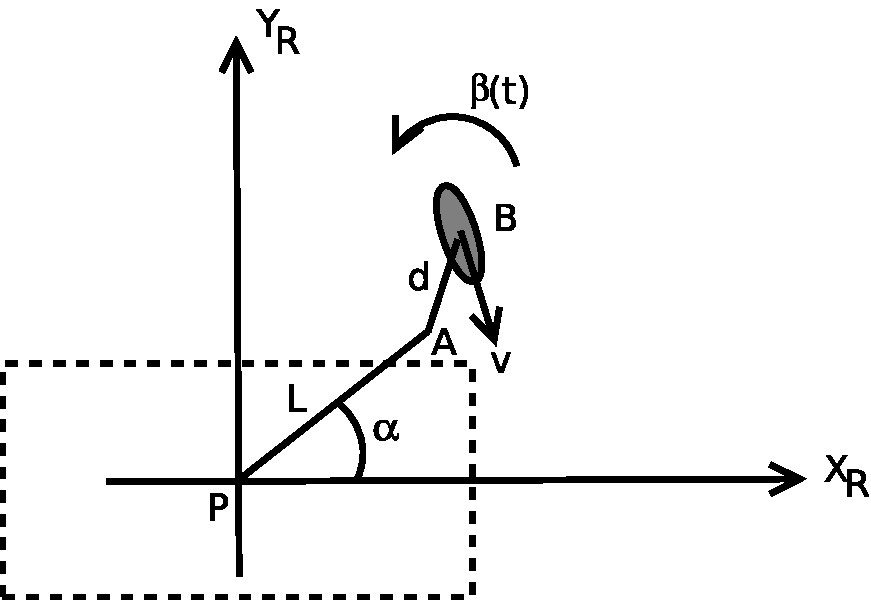
\includegraphics[width=0.4\textwidth,height=\textheight]{KinematicsFigures/castorwheel.*}
\caption{Castor Wheel}
\end{figure}

\hypertarget{omni-swedish-or-mecanum-wheels}{%
\subsection{Omni, Swedish, or Mecanum
Wheels}\label{omni-swedish-or-mecanum-wheels}}

\begin{figure}
\centering
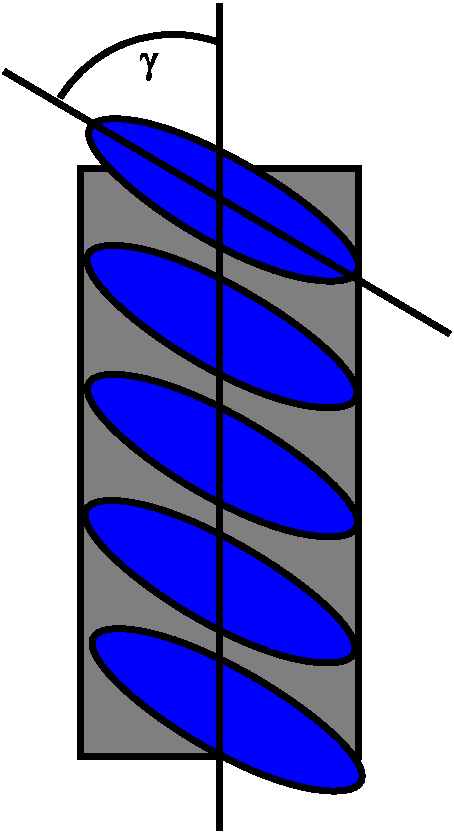
\includegraphics[width=0.15\textwidth,height=\textheight]{KinematicsFigures/swedish_angle.*}
\caption{Swedish Wheel}
\end{figure}

Let \(\gamma\) be the angle between the roller axis and wheel plane
(plane orthogonal to the wheel axis) For \emph{No Slip}:

\begin{quote}
\[\left\langle \sin(\alpha+\beta+\gamma) , -\cos(\alpha+\beta+\gamma), -L\cos(\beta +\gamma) \right\rangle
R(\theta)^{-1}\dot{\xi}_I\]

\(= r\dot{\phi}\cos(\gamma)\)
\end{quote}

For \emph{No Slide}:

\begin{quote}
\[\left\langle \cos(\alpha+\beta +\gamma) , \sin(\alpha+\beta+\gamma),  L\sin(\beta + \gamma) \right\rangle
\cdot R(\theta)^{-1}\dot{\xi}_I\]

\(= r\dot{\phi}\sin(\gamma) + r_{sw}\dot{\phi}_{sw}\)
\end{quote}

\begin{description}
\item[Note that since \(\phi_{sw}\) is free (to spin), the no slide]
condition is not a constraint in the same manner as the fixed or steered
wheels.
\end{description}

\hypertarget{multiple-wheel-model-and-matrix-formulation}{%
\section{Multiple Wheel Model and Matrix
Formulation}\label{multiple-wheel-model-and-matrix-formulation}}

Since nearly all the robots we will work with have three or more wheels.
The equations we derived above can be combined to build a complete
kinematic model. We begin with some basic variables that define the
system.

\begin{itemize}
\tightlist
\item
  Let \(N\) denote the total number of wheels
\item
  Let \(N_f\) denote the number of fixed wheels
\item
  Let \(N_s\) denote the number of steerable wheels
\item
  Let \(\phi_f(t)\) and \(\beta_f\) be the fixed wheel angular velocity
  and wheel position.
\item
  Let \(\phi_s(t)\) and \(\beta_s(t)\) be the steerable wheel angular
  velocity and wheel position.
\end{itemize}

We bundle the latter two values in a vector for notational ease:

\[\phi (t) = ( \phi_{f,1}(t),
\phi_{f,2}(t), \phi_{f,3}(t), ..., \phi_{s,1}(t), \phi_{s,2}(t), ...)\]

\[\beta (t) = ( \beta_{f,1}(t),
\beta_{f,2}(t), \beta_{f,3}(t), ..., \beta_{s,1}(t), \beta_{s,2}(t), ...)\]

Next we collect the no slip constraints, the equations derived above for
the various drive types and place them in a matrix:

\[\begin{aligned}
J_1 R(\theta)^{-1}\dot{\xi}_I = \begin{bmatrix} J_{1f} \\ J_{1s}\end{bmatrix} R(\theta)^{-1} \dot{\xi}_I= J_2 \dot{\phi}
\end{aligned}\]

where \(J_1\) is the matrix with rows made up of the rolling constraints
and \(J_2\) is a diagonal matrix made from wheel diameters. In a similar
manner we can bundle up the no slide constraints (fixed and steered):

\[\begin{aligned}
C_1 R(\theta)^{-1}\dot{\xi}_I = \begin{bmatrix} C_{1f} \\ C_{1s}\end{bmatrix} R(\theta)^{-1} \dot{\xi}_I = 0.
\end{aligned}\]

This is matrix shorthand to address the kinematic models for a variety
of systems.

\[\begin{aligned}
\begin{bmatrix} J_1 \\ C_1 \end{bmatrix} R(\theta)^{-1} \dot{\xi}_I = \begin{bmatrix} J_2 \\ 0\end{bmatrix} \dot{\phi}
\end{aligned}\]
